%%%%%%%%%%%%%%%%%%%%%%%%%%%%%%%%%%%%%%%%%%%%%%%%%%%%%%%%%%%%%%%%%%%%%%%%%%%%%%%%%%%%%%%%%%%%%%
\begin{frame}
  \frametitle{Consistencia, convergencia y estabilidad determinista.}
  \begin{overlayarea}{\textwidth}{.3\textheight}
  \begin{empheq}[box={\Garybox[Errores]}]{align*}
	  \everymath{\scriptstyle}
	  \scriptsize
	  l_{n+1}=&x(t_n;t_n,y_n)-y_{n+1} 		& \text{(local)}\\
	  e_{n+1}=&x(t_{n+1};t_0,x_0)-y_{n+1}	&\text{(global)}
	\end{empheq}
  \end{overlayarea}
  %\begin{columns}
 	%\column{.2\textwidth}
	%\column{.9\textwidth}
	\begin{overlayarea}{\textwidth}{\textheight}
	  \only<+>{
		\begin{center}
		  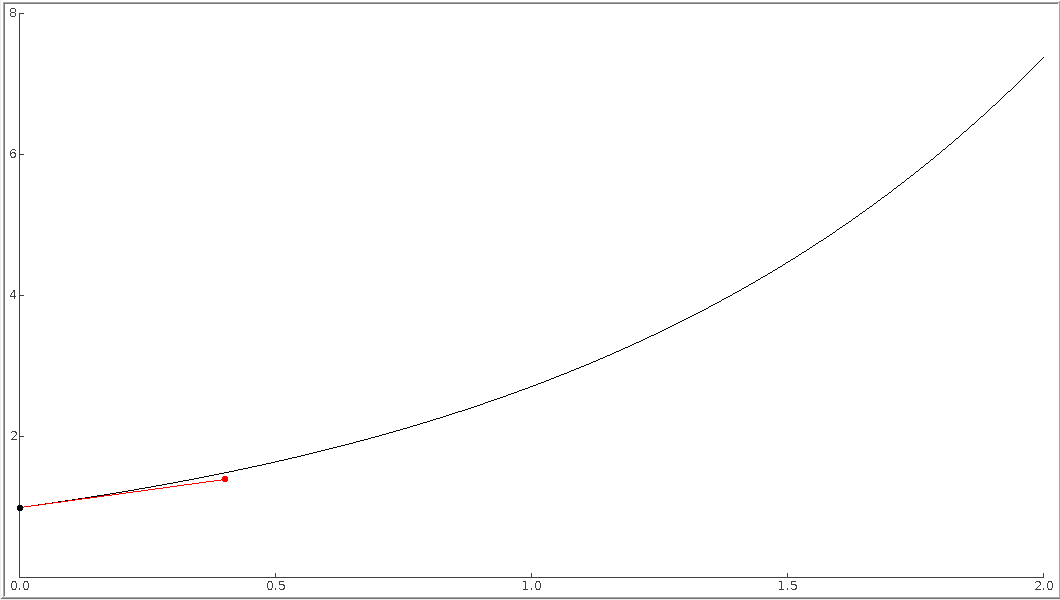
\includegraphics[width=.7\textwidth]{./images/LocalGlobalErrorsA/LocarGlobalErrorA1.png}
		\end{center}
		}
	  \only<+>{
		\begin{center}
		  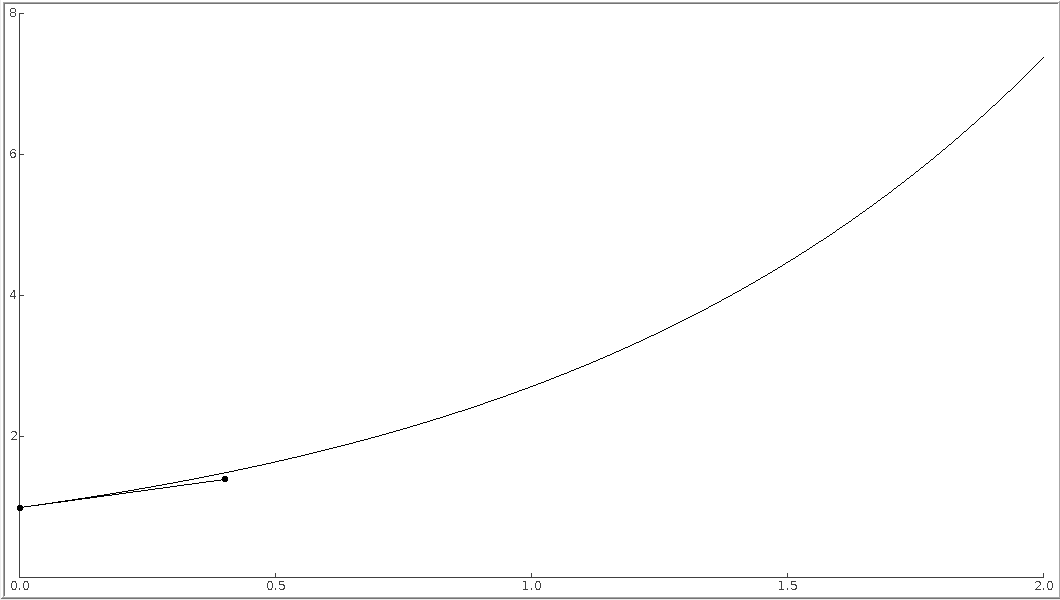
\includegraphics[width=.7\textwidth]{./images/LocalGlobalErrorsA/LocarGlobalErrorA2.png}
		\end{center}
		}
		\only<+>{
		\begin{center}
		  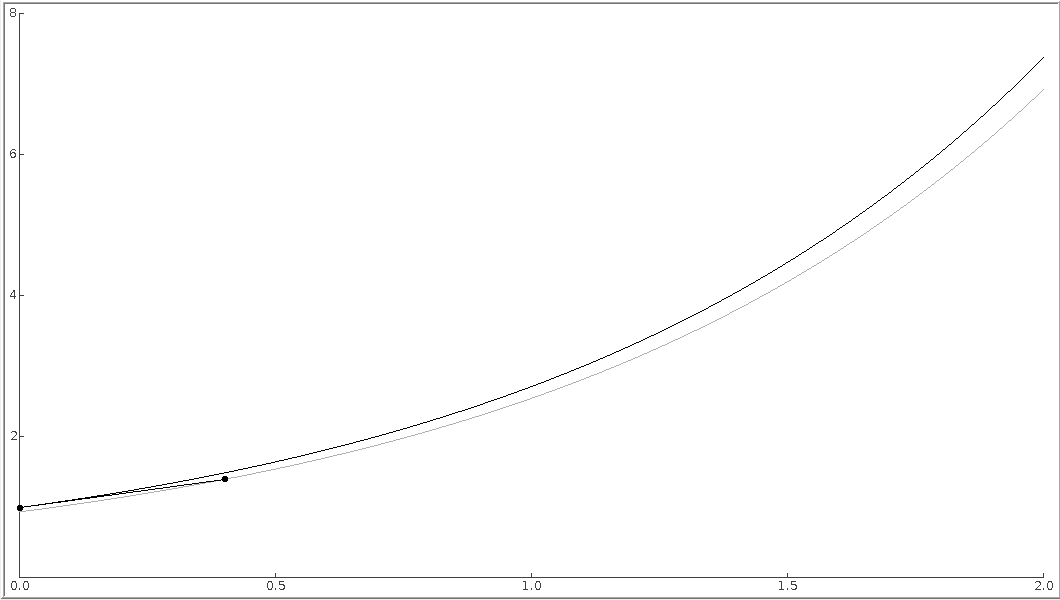
\includegraphics[width=.7\textwidth]{./images/LocalGlobalErrorsA/LocarGlobalErrorA3.png}
		\end{center}
		}
	  \only<+>{
		\begin{center}
		  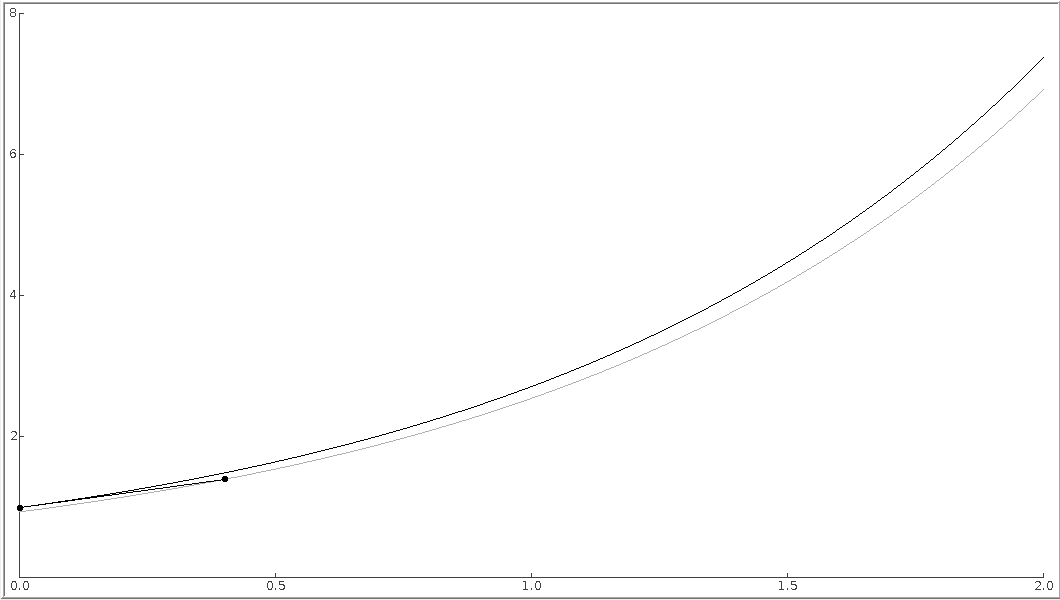
\includegraphics[width=.7\textwidth]{./images/LocalGlobalErrorsA/LocarGlobalErrorA4.png}
		\end{center}
		}
		\only<+>{
		\begin{center}
		  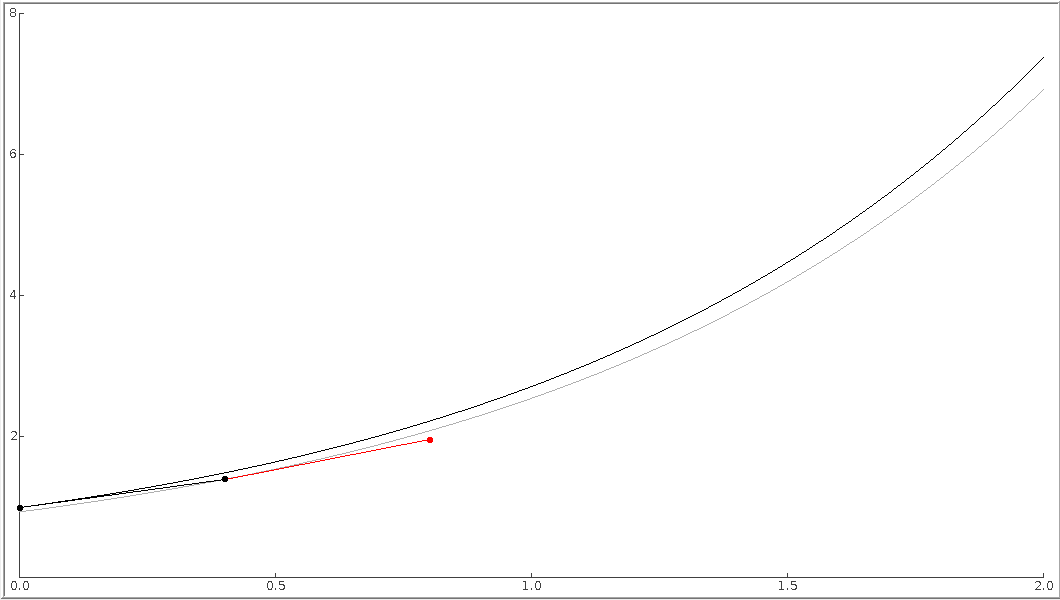
\includegraphics[width=.7\textwidth]{./images/LocalGlobalErrorsA/LocarGlobalErrorA5.png}
		\end{center}
		}
	  \only<+>{
		\begin{center}
		  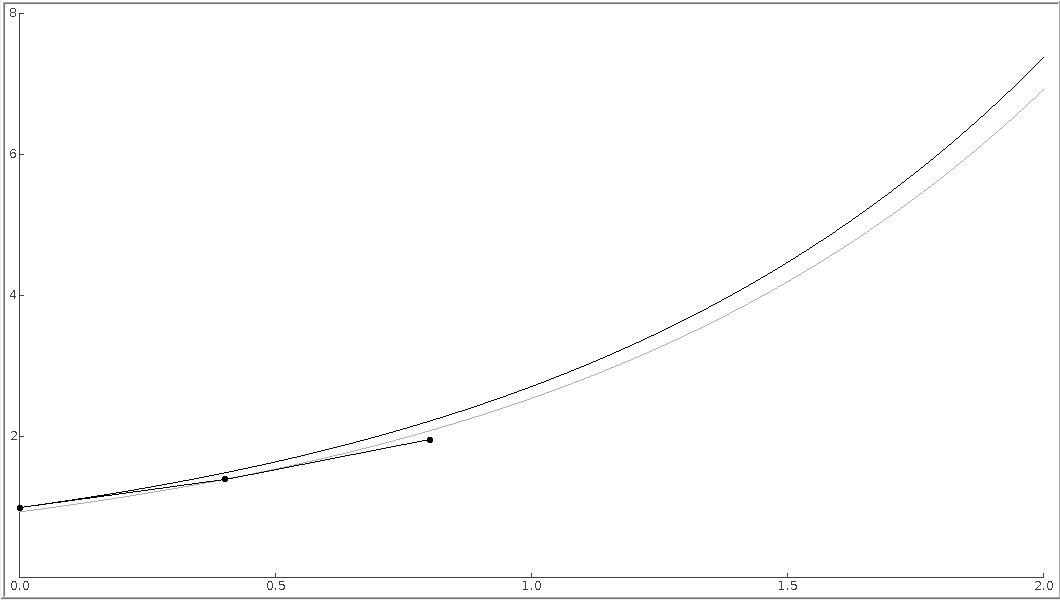
\includegraphics[width=.7\textwidth]{./images/LocalGlobalErrorsA/LocarGlobalErrorA6.png}
		\end{center}
		}
		\only<+>{
		\begin{center}
		  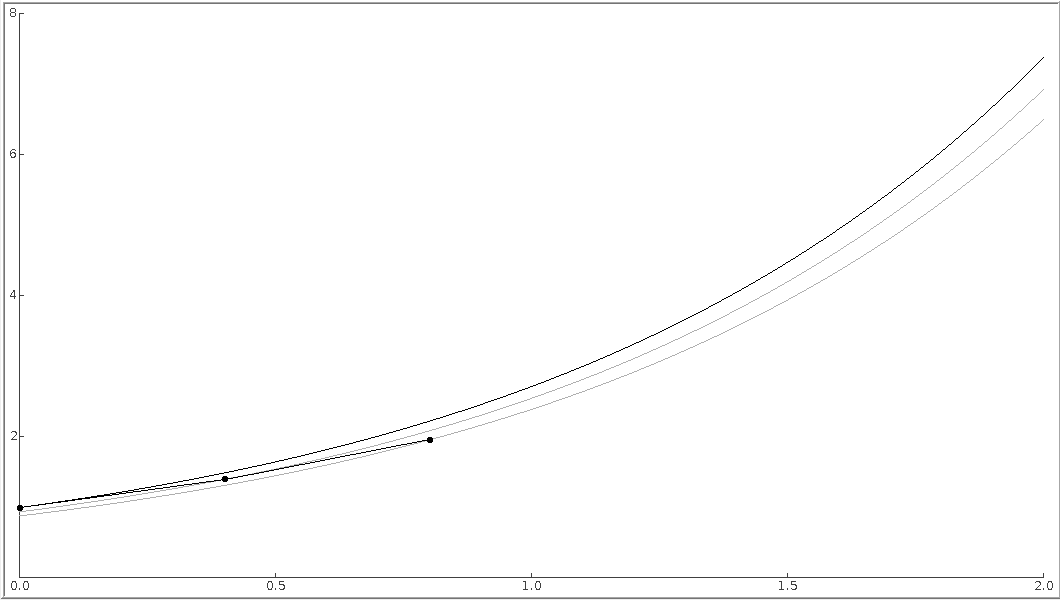
\includegraphics[width=.7\textwidth]{./images/LocalGlobalErrorsA/LocarGlobalErrorA7.png}
		\end{center}
		}
	  \only<+>{
		\begin{center}
		  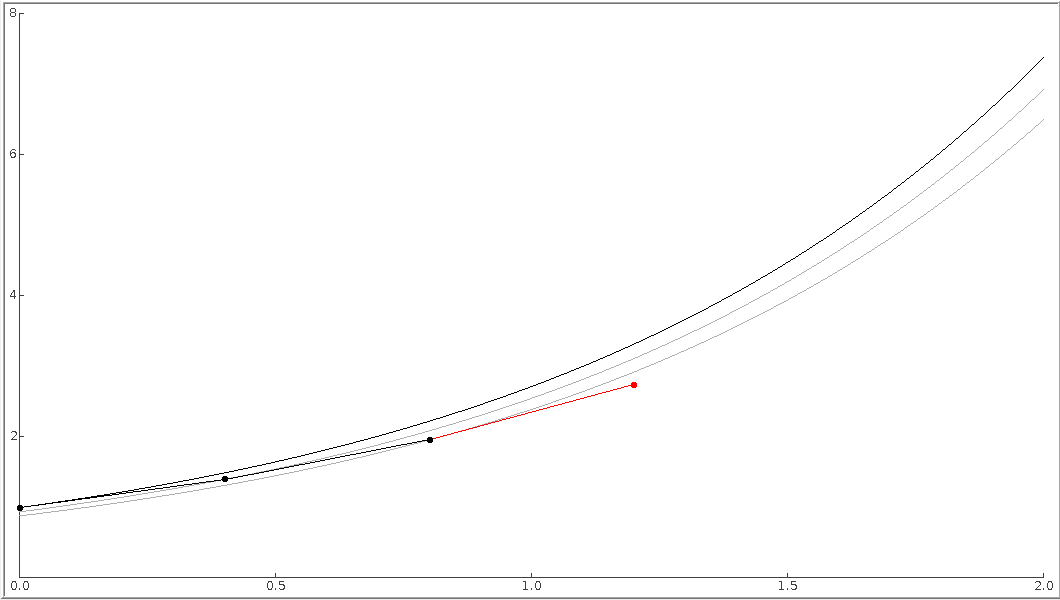
\includegraphics[width=.7\textwidth]{./images/LocalGlobalErrorsA/LocarGlobalErrorA8.png}
		\end{center}
		}
	  \only<+>{
		\begin{center}
		  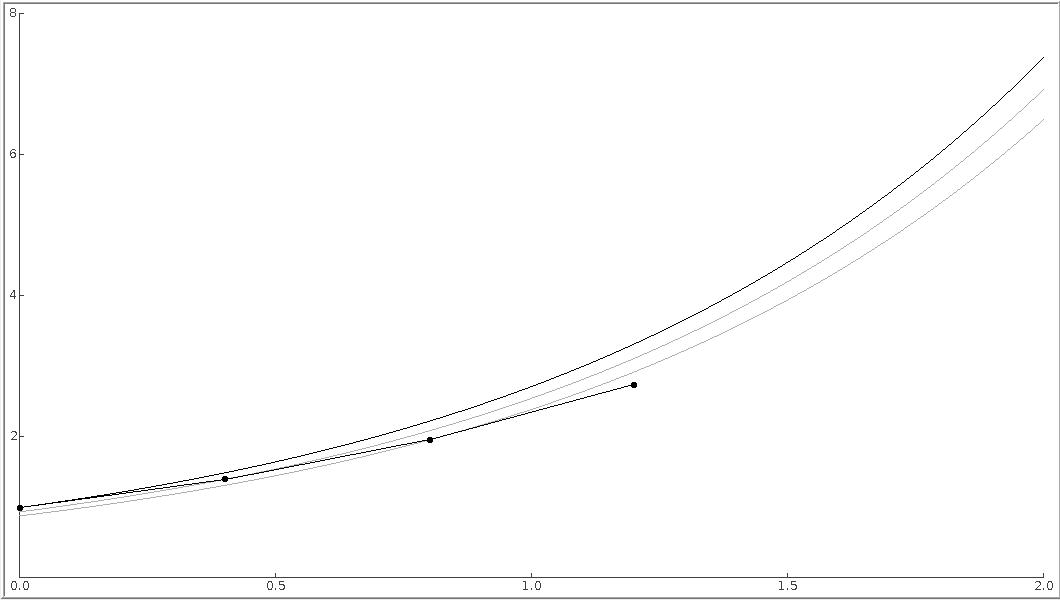
\includegraphics[width=.7\textwidth]{./images/LocalGlobalErrorsA/LocarGlobalErrorA9.png}
		\end{center}
		}
		\only<+>{
		\begin{center}
		  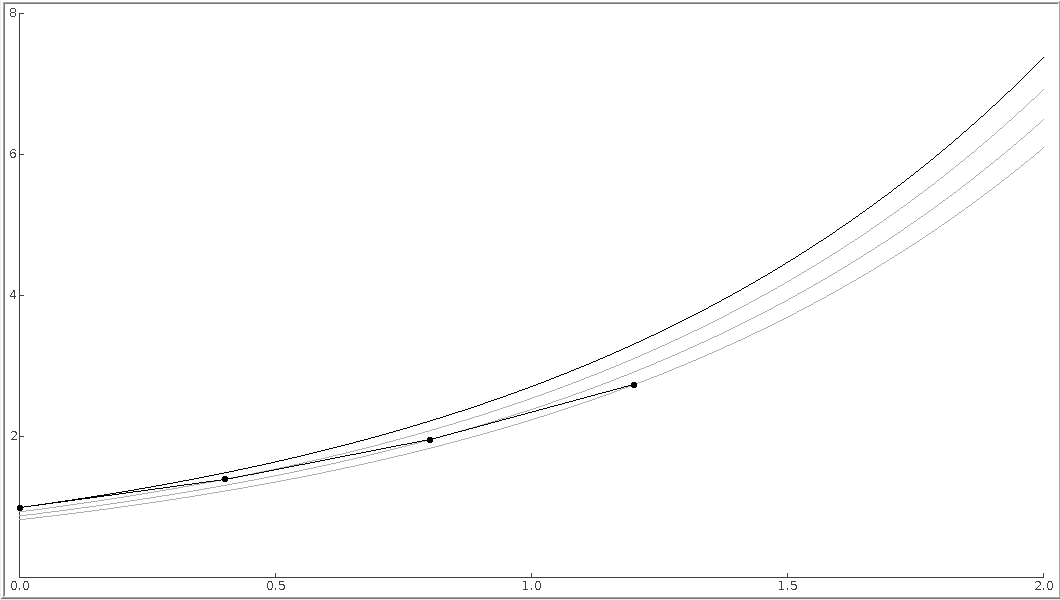
\includegraphics[width=.7\textwidth]{./images/LocalGlobalErrorsA/LocarGlobalErrorA10.png}
		\end{center}
		}
	  \only<+>{
		\begin{center}
		  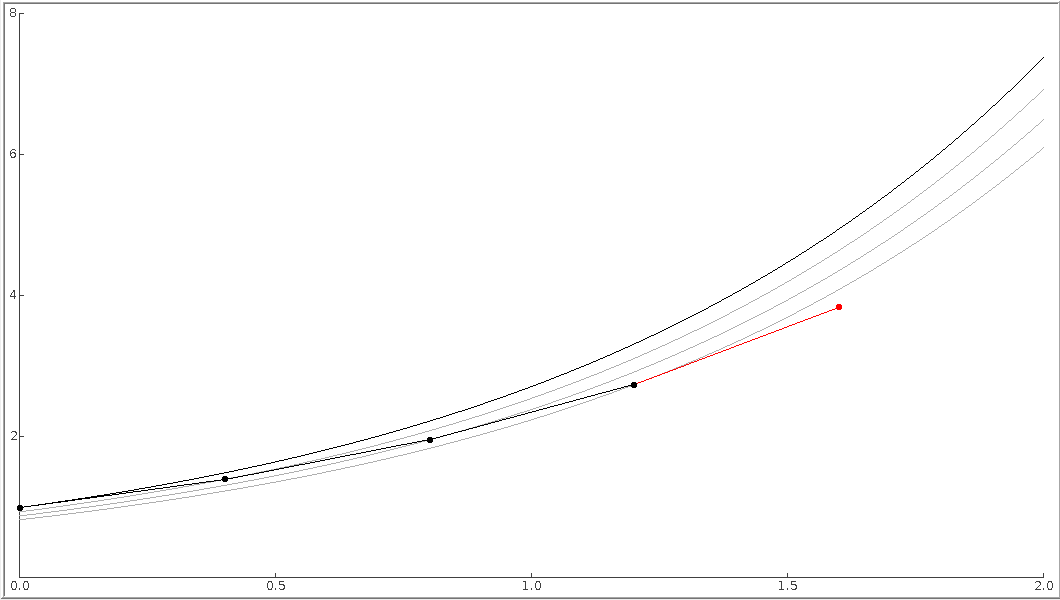
\includegraphics[width=.7\textwidth]{./images/LocalGlobalErrorsA/LocarGlobalErrorA11.png}
		\end{center}
		}
	  \only<+>{
		\begin{center}
		  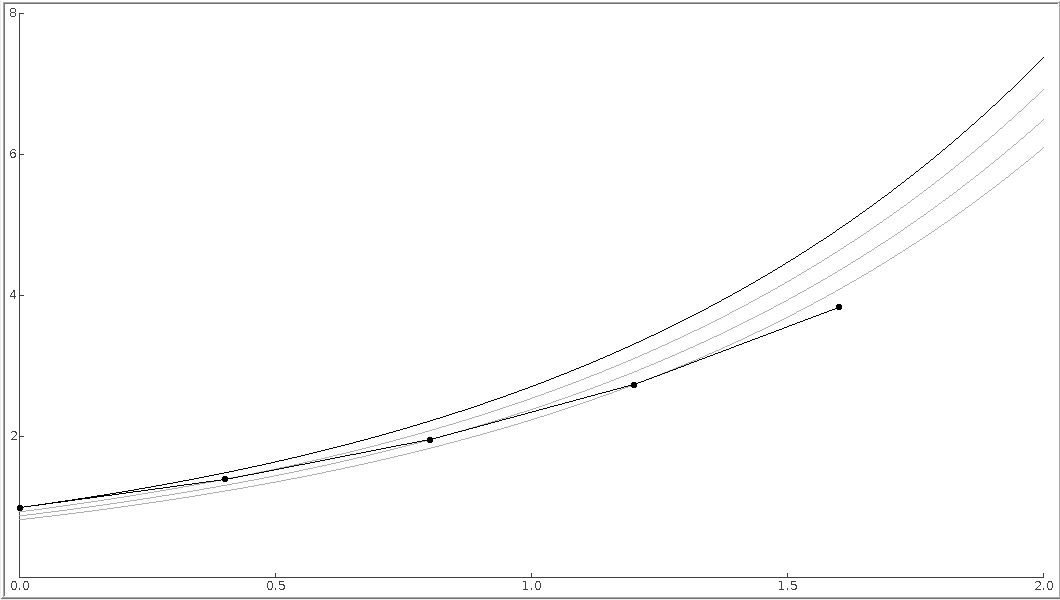
\includegraphics[width=.7\textwidth]{./images/LocalGlobalErrorsA/LocarGlobalErrorA12.png}
		\end{center}
		}
	  \only<+>{
		\begin{center}
		  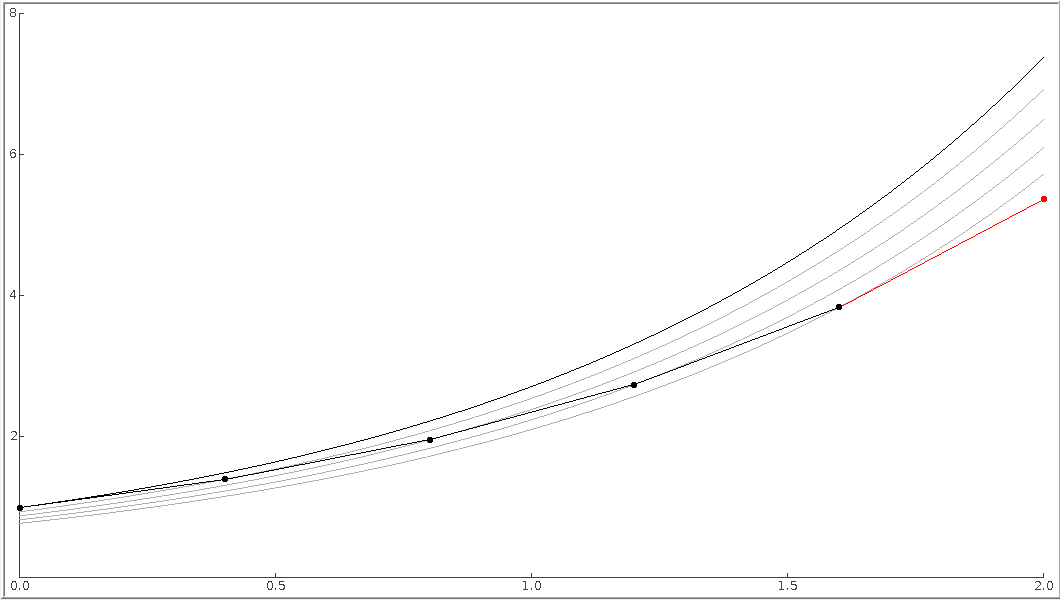
\includegraphics[width=.7\textwidth]{./images/LocalGlobalErrorsA/LocarGlobalErrorA13.png}
		\end{center}
		}
%EjemploB
	  \only<+>{
		\begin{center}
		  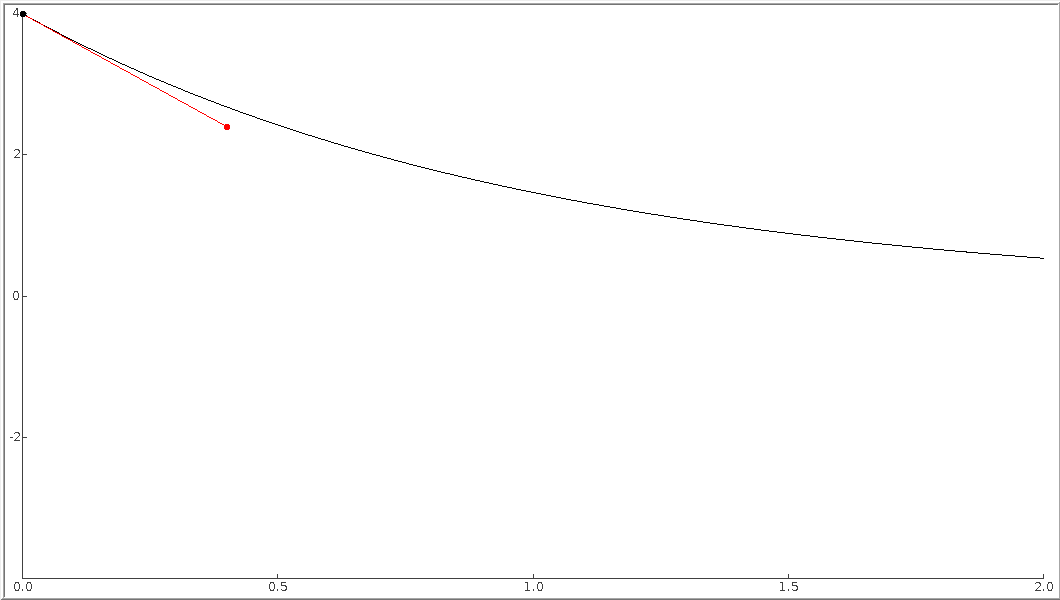
\includegraphics[width=.7\textwidth]{./images/LocalGlobalErrorB/LocarGlobalErrorB1.png}
		  % LocarGlobalErrorB1.png: 1920x1080 pixel, 96dpi, 50.79x28.57 cm, bb=0 0 1440 810
		\end{center}
		}
 		\only<+>{
		\begin{center}
		  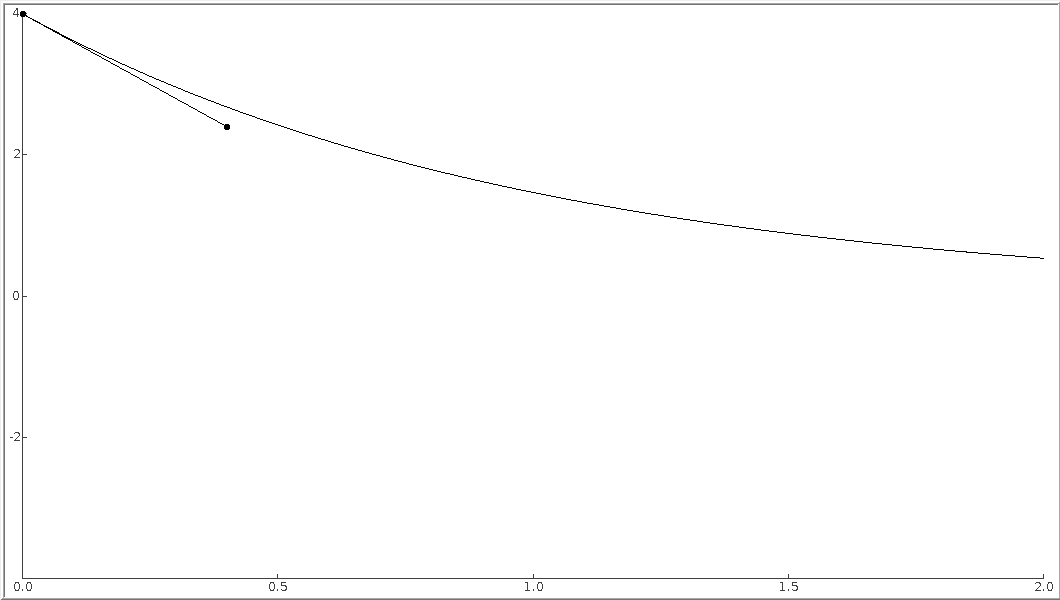
\includegraphics[width=.7\textwidth]{./images/LocalGlobalErrorB/LocarGlobalErrorB2.png}
		  % LocarGlobalErrorB1.png: 1920x1080 pixel, 96dpi, 50.79x28.57 cm, bb=0 0 1440 810
		\end{center}
		}
		\only<+>{
		\begin{center}
		  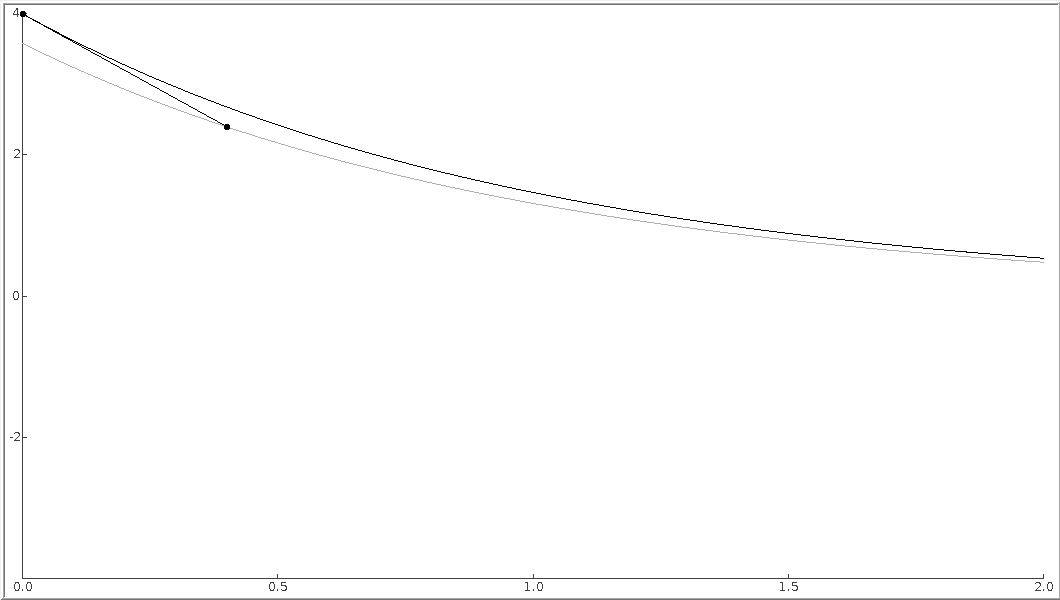
\includegraphics[width=.7\textwidth]{./images/LocalGlobalErrorB/LocarGlobalErrorB3.png}
		  % LocarGlobalErrorB1.png: 1920x1080 pixel, 96dpi, 50.79x28.57 cm, bb=0 0 1440 810
		\end{center}
		}
		\only<+>{
		\begin{center}
		  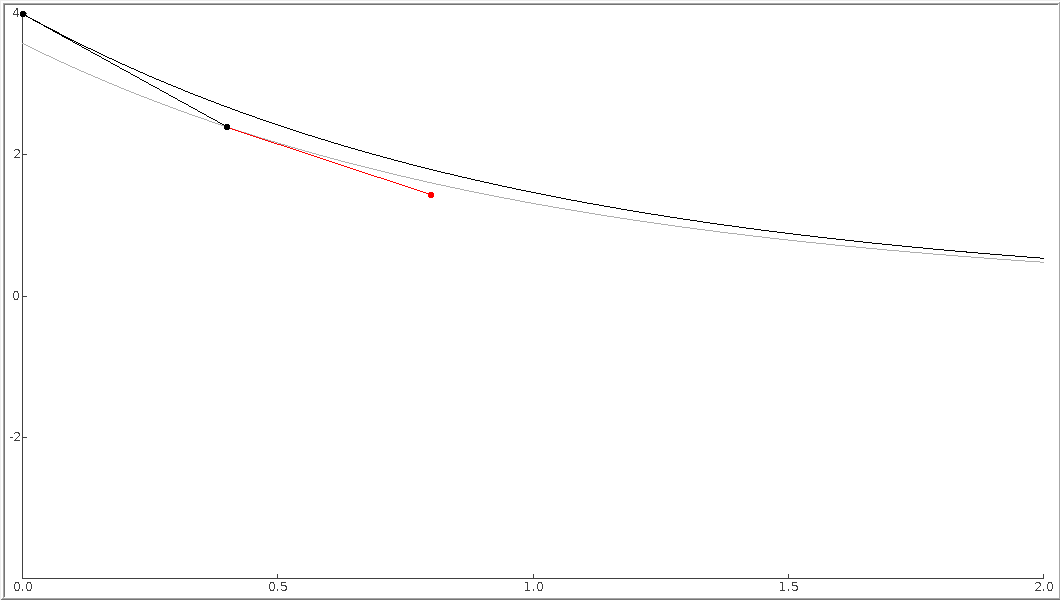
\includegraphics[width=.7\textwidth]{./images/LocalGlobalErrorB/LocarGlobalErrorB4.png}
		  % LocarGlobalErrorB1.png: 1920x1080 pixel, 96dpi, 50.79x28.57 cm, bb=0 0 1440 810
		\end{center}
		}
		\only<+>{
		\begin{center}
		  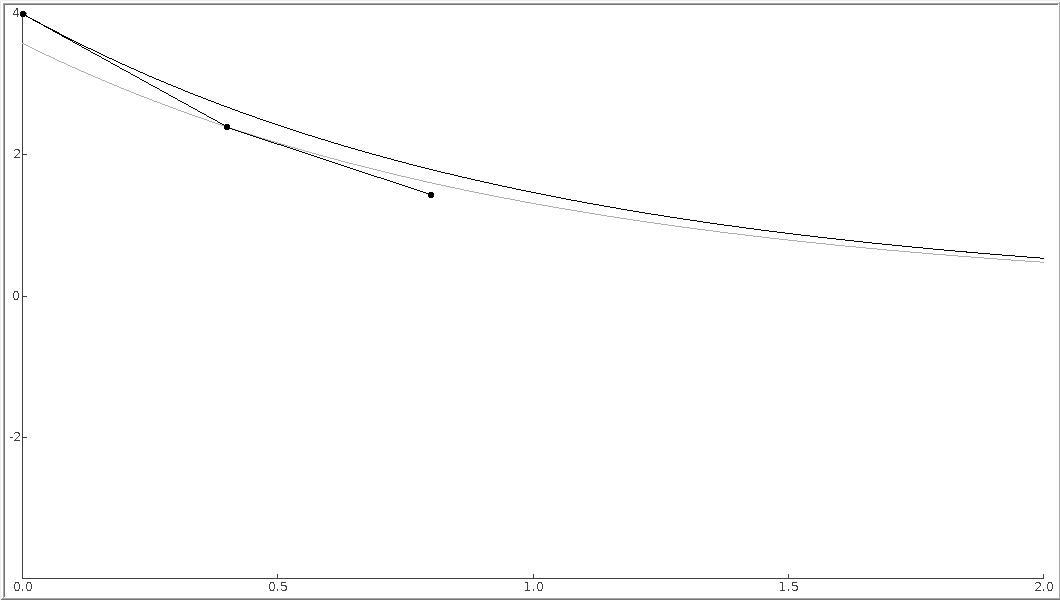
\includegraphics[width=.7\textwidth]{./images/LocalGlobalErrorB/LocarGlobalErrorB5.png}
		  % LocarGlobalErrorB1.png: 1920x1080 pixel, 96dpi, 50.79x28.57 cm, bb=0 0 1440 810
		\end{center}
		}
		\only<+>{
		\begin{center}
		  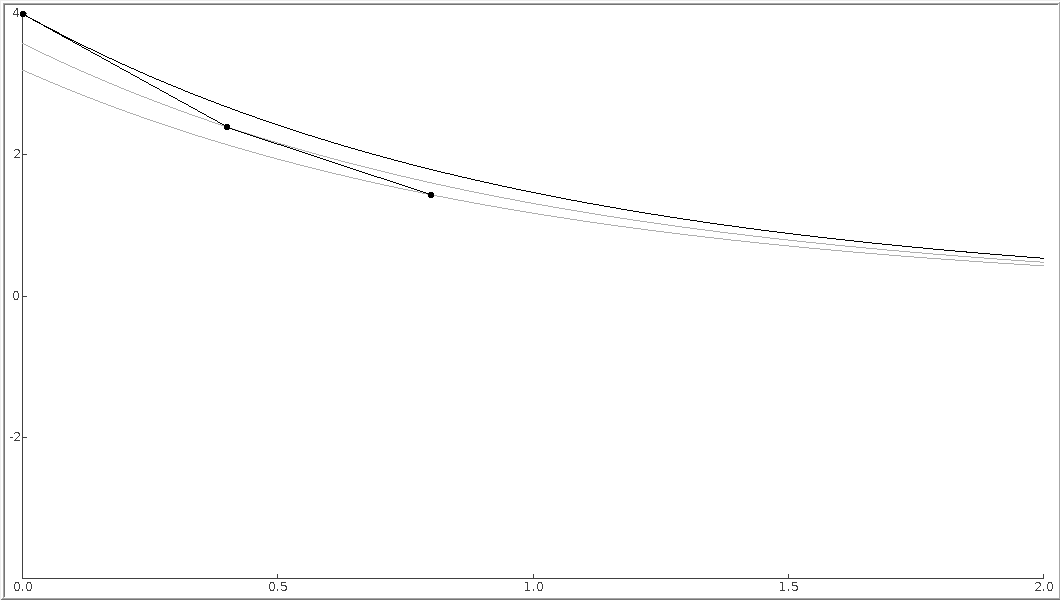
\includegraphics[width=.7\textwidth]{./images/LocalGlobalErrorB/LocarGlobalErrorB6.png}
		  % LocarGlobalErrorB1.png: 1920x1080 pixel, 96dpi, 50.79x28.57 cm, bb=0 0 1440 810
		\end{center}
		}
		\only<+>{
		\begin{center}
		  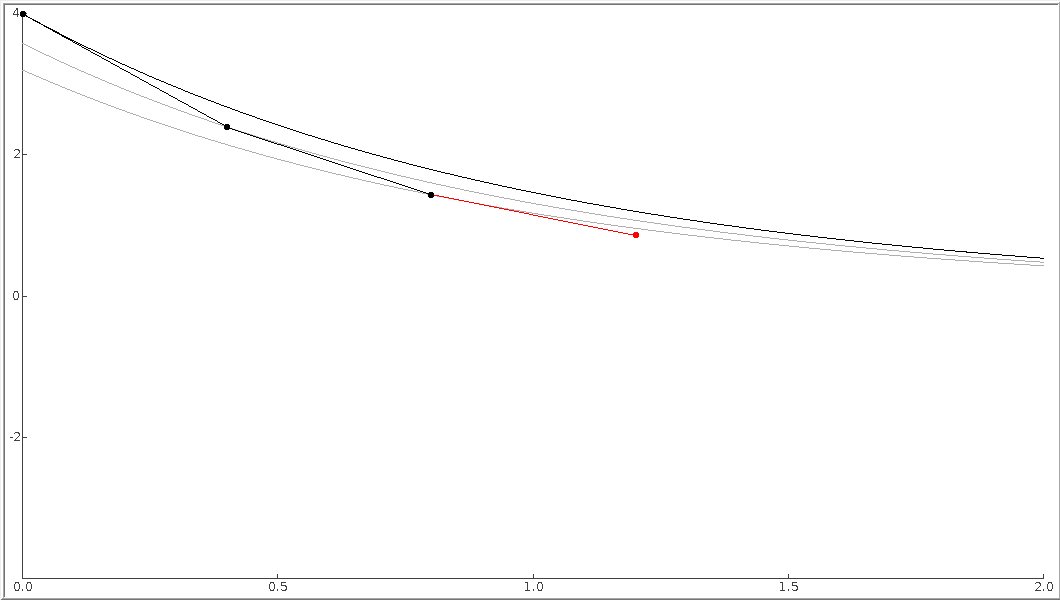
\includegraphics[width=.7\textwidth]{./images/LocalGlobalErrorB/LocarGlobalErrorB7.png}
		  % LocarGlobalErrorB1.png: 1920x1080 pixel, 96dpi, 50.79x28.57 cm, bb=0 0 1440 810
		\end{center}
		}
		\only<+>{
		\begin{center}
		  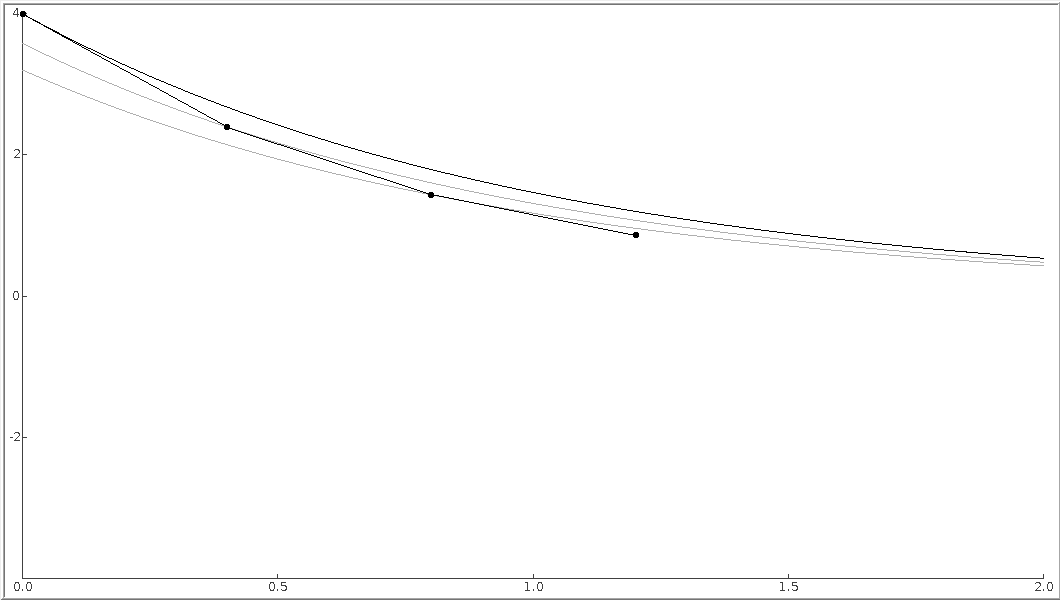
\includegraphics[width=.7\textwidth]{./images/LocalGlobalErrorB/LocarGlobalErrorB8.png}
		  % LocarGlobalErrorB1.png: 1920x1080 pixel, 96dpi, 50.79x28.57 cm, bb=0 0 1440 810
		\end{center}
		}
		\only<+>{
		\begin{center}
		  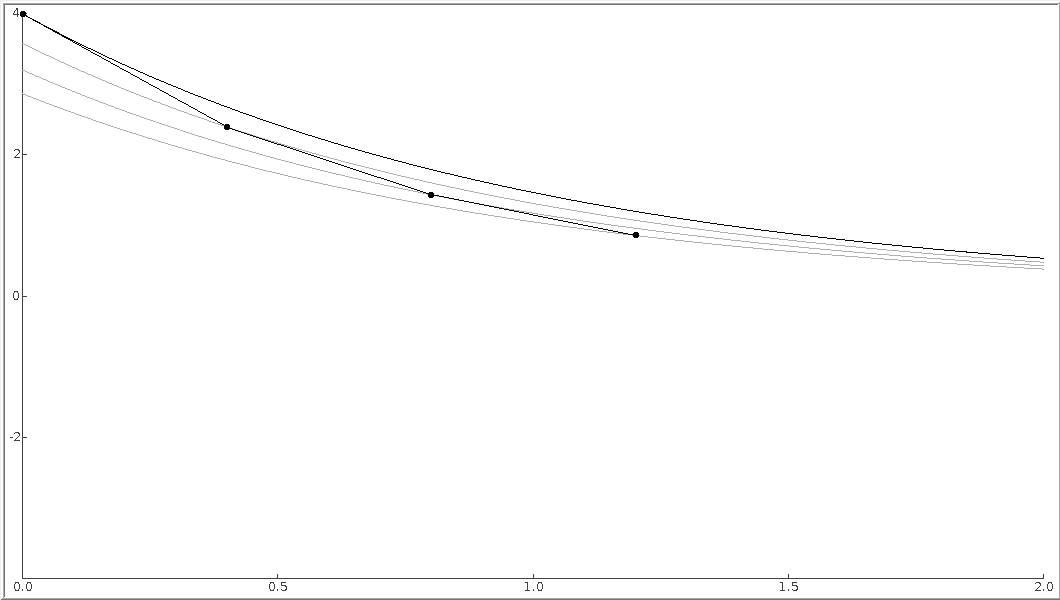
\includegraphics[width=.7\textwidth]{./images/LocalGlobalErrorB/LocarGlobalErrorB9.png}
		  % LocarGlobalErrorB1.png: 1920x1080 pixel, 96dpi, 50.79x28.57 cm, bb=0 0 1440 810
		\end{center}
		}
		\only<+>{
		\begin{center}
		  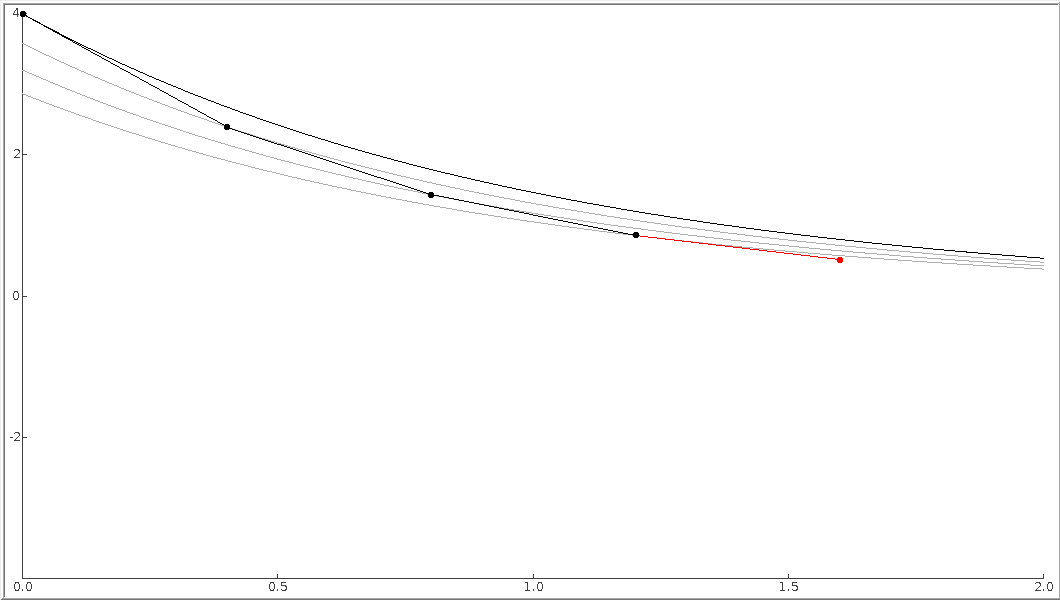
\includegraphics[width=.7\textwidth]{./images/LocalGlobalErrorB/LocarGlobalErrorB10.png}
		  % LocarGlobalErrorB1.png: 1920x1080 pixel, 96dpi, 50.79x28.57 cm, bb=0 0 1440 810
		\end{center}
		}
		\only<+>{
		\begin{center}
		  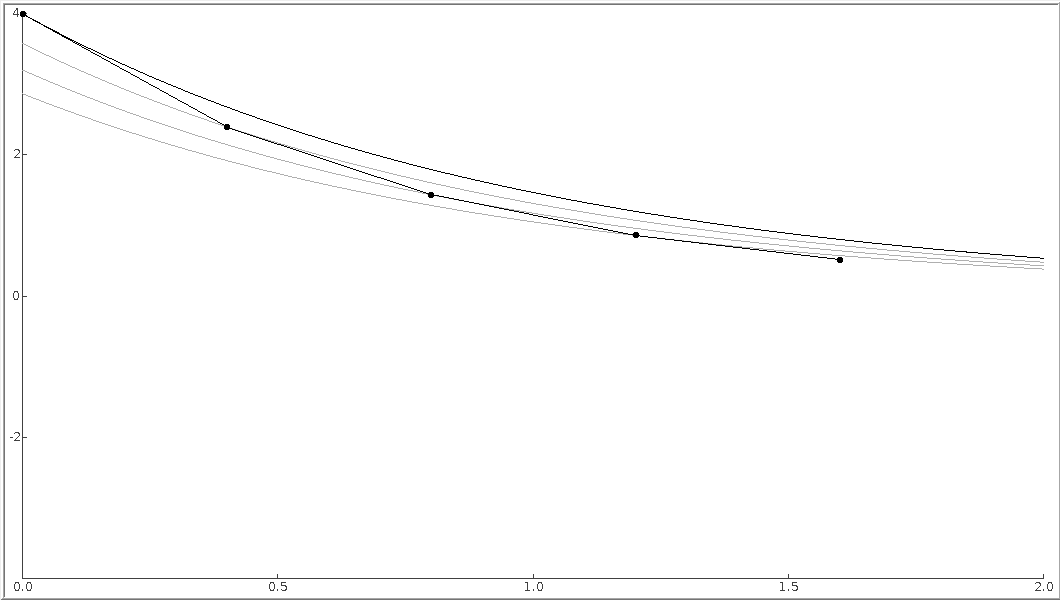
\includegraphics[width=.7\textwidth]{./images/LocalGlobalErrorB/LocarGlobalErrorB11.png}
		  % LocarGlobalErrorB1.png: 1920x1080 pixel, 96dpi, 50.79x28.57 cm, bb=0 0 1440 810
		\end{center}
		}
		\only<+>{
		\begin{center}
		  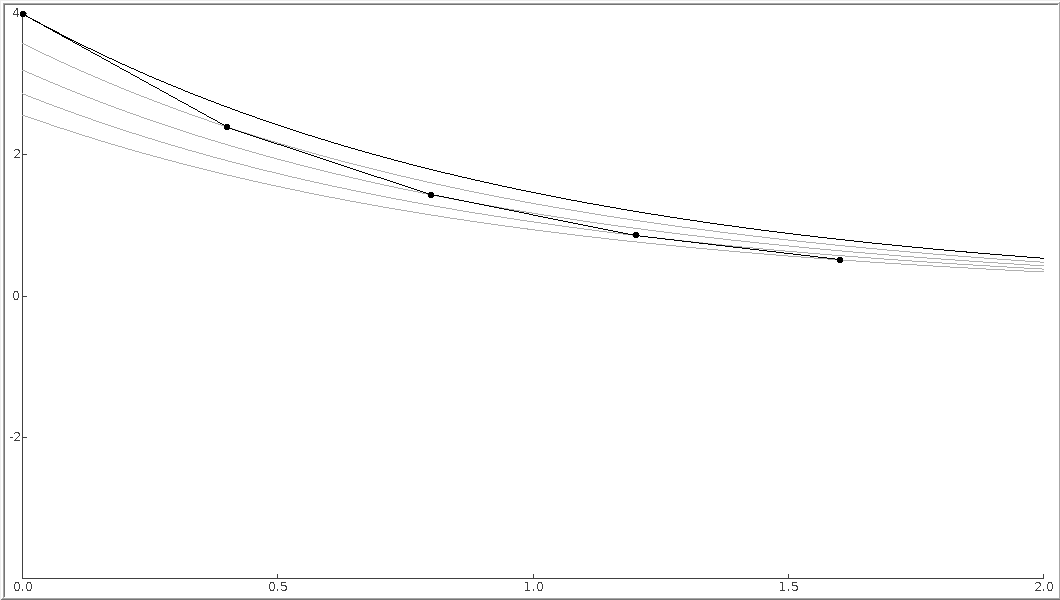
\includegraphics[width=.7\textwidth]{./images/LocalGlobalErrorB/LocarGlobalErrorB12.png}
		  % LocarGlobalErrorB1.png: 1920x1080 pixel, 96dpi, 50.79x28.57 cm, bb=0 0 1440 810
		\end{center}
		}
		\only<+>{
		\begin{center}
		  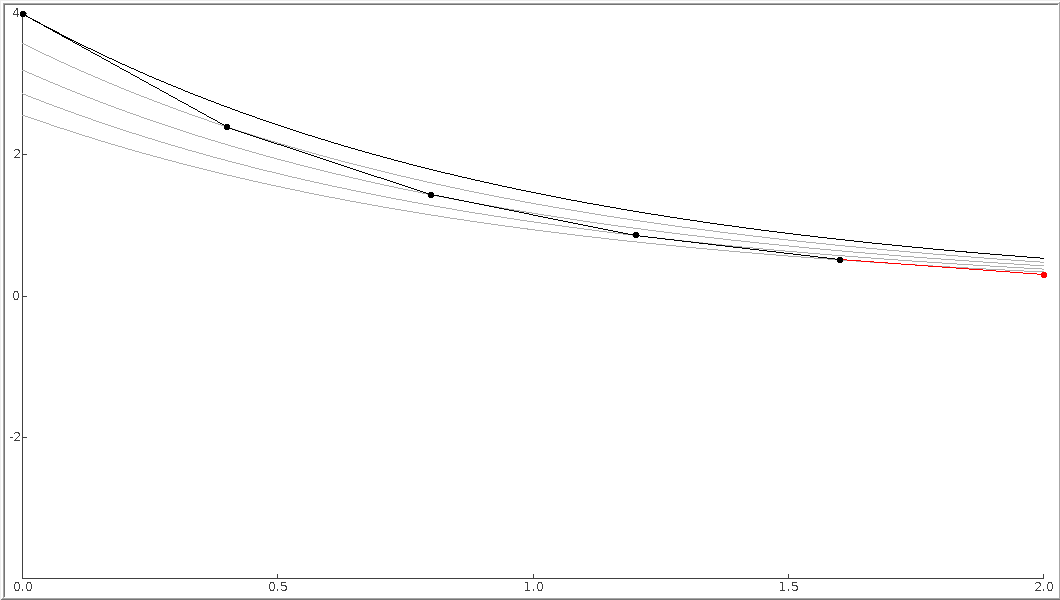
\includegraphics[width=.7\textwidth]{./images/LocalGlobalErrorB/LocarGlobalErrorB13.png}
		  % LocarGlobalErrorB1.png: 1920x1080 pixel, 96dpi, 50.79x28.57 cm, bb=0 0 1440 810
		\end{center}
		}
	\end{overlayarea}
%\end{columns}
\end{frame}
%%%%%%%%%%%%%%%%%%%%%%%%%%%%%%%%%%%%%%%%%%%%%%%%%%%%%%%%%%%%%%%%%%%%%%%%%%%%%%%%%%%%%%%%%%%%%%%%%
\begin{frame}
	\begin{overlayarea}{\textwidth}{.5\textheight}
	  \begin{empheq}[box=\shadowbox]{equation*}
	  \frac{dx}{dt}=a(t,x), \qquad y_{n+1}=y_n+\Psi(t_n,y_n,h_n)h_n
	\end{empheq}
	\begin{columns}
	  \column{.5\textwidth}
		\only<3->{
		\begin{Teorema}
		  Si $\Psi$ satisface
		  \begin{itemize}
			\item
			%$\displaystyle |\Psi(t',x',\Delta')-\Psi(t,x,\Delta)|\leq K(|t'-t|+|x'-x|+|\Delta'-\Delta|)$
			(Lipschitz en $(t,x,h)$)
		  \item
			%$|\Psi(t,x,0)|\leq L \quad \forall (t,x)$
			(Acotada)
		\end{itemize}
		entonces  convergente $\Leftrightarrow$ consistente.
	  \end{Teorema}
	  }
	  \column{.5\textwidth}
	  \only<5->{
	  \vspace{-.3cm}
	  \begin{Teorema}
	  	\begin{empheq}[ innerbox=\fbox, right=\Rightarrow Estabilidad ]{align*}
			Consistencia\\ 
			Convergencia
		\end{empheq}
		
	  \end{Teorema}
	  }
	\end{columns}
  \end{overlayarea}
	\begin{columns}
	\column{.5\textwidth}
	\begin{overlayarea}{\textwidth}{\textheight}
	  \only<1-2>{
	  \begin{definicion}[Consistencia]
		$$
		  \Psi(t,x,0)=a(t,x).
		$$
	  \end{definicion}
	  }
	\only<6->{
		\vspace{1cm}
			\begin{definicion}[NAE]
				$$
					\lim_{n\to\infty}
					|y_n-\tilde{y}_n|\leq M|y_0-\tilde{y}_0|
				$$			
			\end{definicion}	  
	  }	
	\end{overlayarea}
	\column{.5\textwidth}
	  \begin{overlayarea}{\textwidth}{\textheight}
	  \only<2>{
	  \begin{definicion}[Convergencia]
		$$
		  \lim_{\Delta \downarrow 0} |e_{n+1}|=0
		$$
	  \end{definicion}
	  }
	  \only<4->{
		\vspace{.70cm}
		\begin{definicion}[numéricamente estable]
		  Dados $[t_0,T]$ y (EDO), $\exists h_0,M$ t.q.
		  $$
			|y_n-\tilde{y}_n|\leq M|y_0-\tilde{y}_0| 
			%n=0,1,\dots,n_{T}\\
			%\max_{n} h_{n} <h_0.
		  $$
		 \end{definicion} 
	  }
	\end{overlayarea}
  \end{columns}
\end{frame}
